\documentclass{beamer}
\usepackage[ utf 8]{ inputenc }
\usepackage[serbian]{babel}
\usetheme{CambridgeUS}
\setbeamercolor{item projected}{bg=red}
\setbeamercolor{caption name}{fg=red}
\usepackage{fancybox,graphicx}

\title{Reklame na društvenim mrežama}
\author[Maksimović,Pavlićević,Marković,Damnjanović  ]{Teodora Maksimović\\Natalija Pavlićević\\
	Branka Marković\\Mihailo~Damnjanović}
\institute[]{Matematički fakultet, Univerzitet u Beogradu}
\date{4.11.2022.}
\begin{document}
	
	\frame{\titlepage}
	
	\begin{frame}{Prikupljanje podataka korisnika u cilju personalizovanog oglašavanja}
		\begin{itemize}
			\item Ciljano reklamiranje postaje sve važniji izvor prihoda i za oglašivače i za reklamne kompanije.
			\item Podaci koje pružaju korisnici omogućavaju onlajn provajderima društvenih medija da personalizaciju svog sadržaja
			\item Personalizacijom se cilja na relevantniji oglasni sadržaj i ostvarivanje većeg profita za oglašivače.
		\end{itemize}
	\end{frame}
	
	\begin{frame}{Prikupljanje podataka korisnika u cilju personalizovanog oglašavanja}
		\begin{itemize}
			\item Okupljeni podaci se obrađuju i analiziraju zarad postizanja smislenih informacija.
			\item Koristeći podatke klasifikuju se tipovi korisnika. \item Sadržane ključne reči igraju glavnu ulogu u oglašavanju ciljanoj grupi ljudi.
		\end{itemize}
		
	\end{frame}
	
	\begin{frame}
		\frametitle{Algoritmi u odabiru reklama}
		\begin{itemize}
			\item Trag na internetu
			\item Konstantan priliv podataka u sistem koji je potpuno mašinski osamostaljen
			\item Algoritam društvenih medija bira oglase za koje misli da će korisnici biti zainteresovani, na osnovu prikupljenih podataka
		\end{itemize} 
	\end{frame}
	
	\begin{frame}
		\begin{itemize}
			\item Određene platforme nam pružaju mogućnost da vidimo zašto su nam prikazale baš taj oglas. Primer za to je Fejsbuk (eng.~{\em Facebook}) :
		\end{itemize}
		\begin{figure}[h!]
			\begin{center}
				\shadowbox{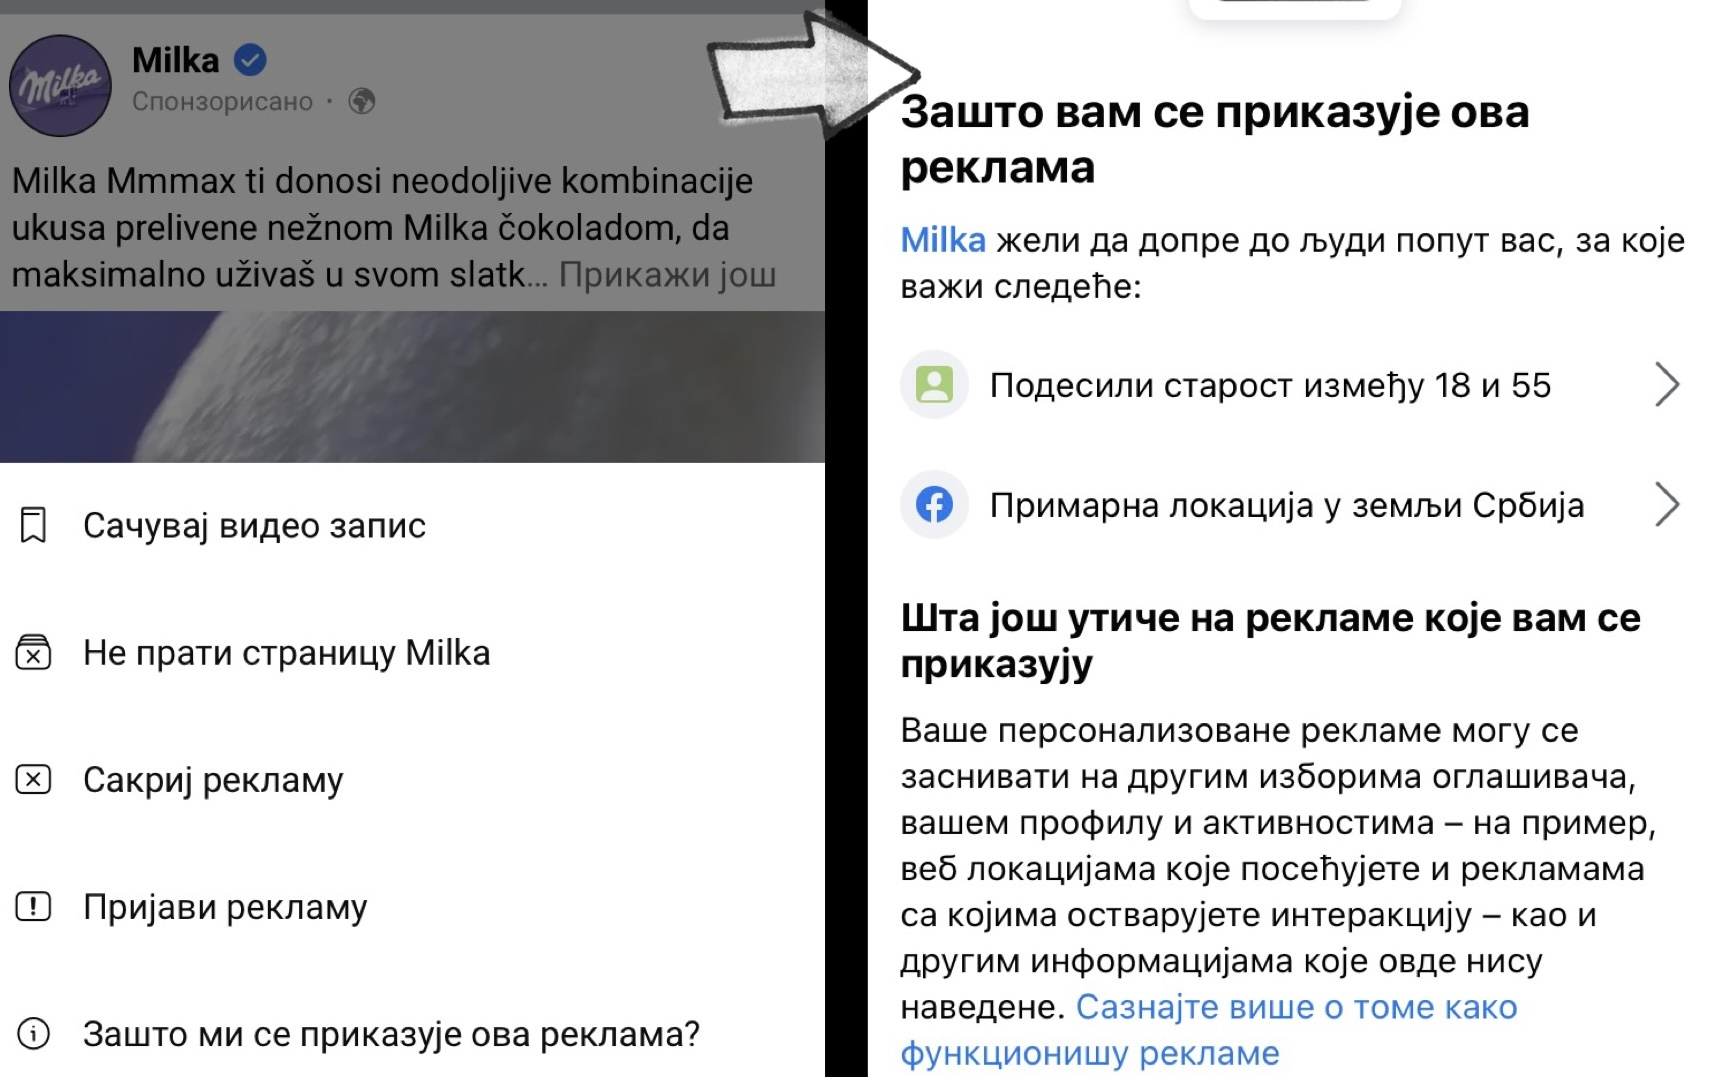
\includegraphics[scale=0.15]{zastoreklama.jpg}}
			\end{center}
		\end{figure}
	\end{frame}
	
	\begin{frame}{Kako ovaj algoritam doprinosi uspešnosti reklama?}
		\begin{itemize}
			\item Od 10\% do 30\% veći profit za oglašivače
			\item Doprinosi impulsivnoj kupovini
			\item Smanjenje vraćanja robe
			\item Povećanje lojalnosti usled personalizovanog iskustva
		\end{itemize}
	\end{frame}
	
	\begin{frame}{Mišljenje korisnika o reklamama na internetu}
		\begin{itemize}
			\item Mišljenja korisnika se razlikuju.
			\item Reklame smetaju korisnicima u korišcenju interneta.
			\item Korisnike interesuju reklame, uglavnom kada tragaju za nekim proizvodom.
			\item Da li korisnici veruju reklamama na internetu?
			\item Social Serbia 2020 je sprovela istraživanje koje pokazuje u kom procentu korisnici veruju reklamama.
		\end{itemize}
		\begin{table}[h!]
			\begin{center}
				\caption{Verovanje reklamama}
				\begin{tabular}{|c|c|} \hline
					Da, verujem&9\%\\ \hline
					Da, ali samo reklamama brendova koje poznajem&29\%\\ \hline
					Da, ali samo ako su mi relevantna i pronalazim se u njima&37\%\\ \hline
					Ne verujem reklamama na internetu&25\%\\ \hline
				\end{tabular}
				\label{tab:tabela1}
			\end{center}
		\end{table}
	\end{frame}
	
	
	\begin{frame}{Koliko često korisnici klikću na reklame?}
		
		\begin{itemize}
			\item Social Serbia 2020 je sprovela istraživanje koliko cesto korisnici kliknu na reklame i to se može videti na slici
			\begin{figure}[h!]
				\begin{center}
					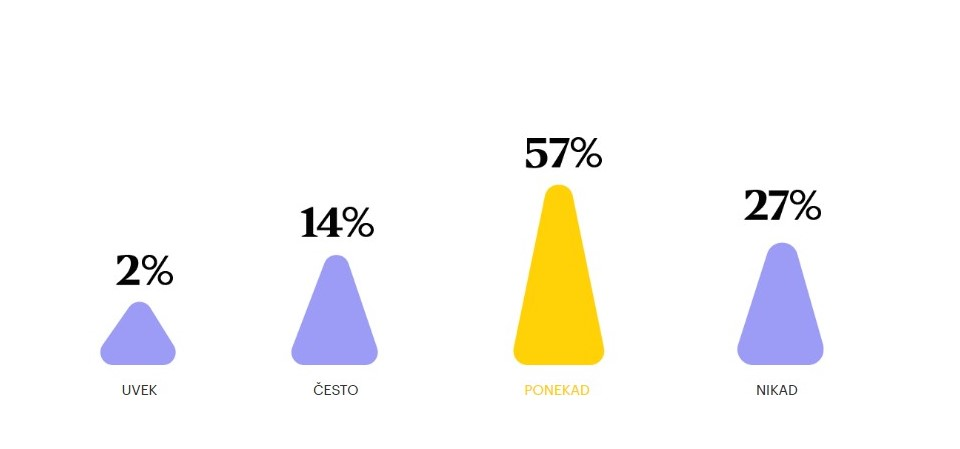
\includegraphics[scale=0.40]{klik_na_reklamu.jpg}
				\end{center}
				\caption{Prikaz učestalosti i akcije na ponuđenu reklamu}
				\label{fig:klik_na_reklamu}
			\end{figure}
		\end{itemize}
		
	\end{frame}
	
	\begin{frame}{Doprinos od reklama}
		\begin{itemize}
			\item Hubspot marketing statistics sproveo je istraživanje o koliko su reklame bitne i o tome govore sledeći podaci:
			\item 84\% marketing stručnjaka se reklamira na nekoj društvenoj mreži
			\item 83\% njih insistira da su društvene mreže bitne za njihov biznis
			\item Broj preduzetnika koji tvrde da je Facebook neophodan za njihov biznis je skocio na 75\%
			\item Društvene mreže su dovele do značajnog porasta stope koverzije u poređenju sa tradicionalnim marketingom 
		\end{itemize}
	\end{frame}
	
\end{document}